\documentclass{beamer}
\usepackage{listings}
\lstset{
%language=C,
frame=single, 
breaklines=true,
columns=fullflexible
}
\usepackage{blkarray}
\usepackage{subcaption}
\usepackage{url}
\usepackage{tikz}
\usepackage{tkz-euclide} % loads  TikZ and tkz-base
%\usetkzobj{all}
\usetikzlibrary{calc,math}
\usepackage{float}
\providecommand{\brak}[1]{\ensuremath{\left(#1\right)}}
\providecommand{\pr}[1]{\ensuremath{\Pr\left(#1\right)}}
\newcommand{\myvec}[1]{\ensuremath{\begin{pmatrix}#1\end{pmatrix}}}
\newcommand\norm[1]{\left\lVert#1\right\rVert}
\renewcommand{\vec}[1]{\mathbf{#1}}
\usepackage[export]{adjustbox}
\usepackage[utf8]{inputenc}
\usepackage{amsmath}
\usepackage{tikz}
\usetikzlibrary{automata, positioning}
\usetheme{Boadilla}

\title{GATE-EC 2016 Q.33}
\author{Nelakuditi Rahul Naga - AI20BTECH11029}
\begin{document}

\begin{frame}
\titlepage
\end{frame}

\begin{frame}
\frametitle{Question}
\begin{block}{GATE-EC 2016 Q.33}
The Discrete Fourier Transform (DFT) of the 4 point sequence $ x[n]$ = $\{3, 2, 3, 4\}$ is given by $ X[k] =\{12, 2j, 0, -2j\}$. If $X_{1}[k]$ is the DFT of the 12 point sequence $ x_{1}[n] =\{3, 0, 0, 2, 0, 0, 3, 0, 0, 4, 0, 0\}$ , find the value of $\big|{\frac{X_{1}[8]}{X_{1}[11]}}\big|$.
\end{block}
\end{frame}

\begin{frame}
\frametitle{Solution}
\begin{block}{4-point DFT matrix}
The 4-point DFT matrix is given by:
\begin{align}
\vec{W_{4}} &=\myvec{
 1  & 1 & 1 & 1 \\
 1 & \omega^1  &\omega^2  &\omega^3  \\
 1 & \omega^2  &\omega^4  &\omega^6  \\
 1 & \omega^3  &\omega^6  &\omega^9 }\\
&=\myvec{
1 &  1 &  1 &  1\\
1 &  -j & -1 & j\\
1 & -1 &  1 & -1\\
1 & j & -1 & -j}
\end{align}
where $\omega = e^{\dfrac{-2 \pi j}{4}} = -j.$
\end{block}
\end{frame}

\begin{frame}
\frametitle{}
Now from the given information we can write:
\begin{align}
\vec{X} = \vec{W_{4}}\vec{x} \label{eq:1}
\end{align}
where
\begin{align}
\vec{x} &=\myvec{3 \\ 2 \\ 3 \\ 4 }
\end{align}
and 
\begin{align}
\vec{X}&=\myvec{12 \\ 2j \\ 0 \\ -2j}  
\end{align}
Now we need to find $\vec{X_{1}}$ satisfying the relation :
\begin{align}
\vec{X_{1}} = \vec{W_{12}}\vec{x_{1}} \label{eq:2}  
\end{align}
\end{frame}

\begin{frame}
\frametitle{}
where
\begin{align}
\vec{x_{1}} &=\myvec{3 \\ 0 \\ 0 \\ 2 \\ 0 \\ 0 \\ 3 \\ 0 \\ 0 \\ 4 \\ 0 \\ 0}
\end{align}
and $\vec{W_{12}}$ is the 12-point DFT matrix.
\end{frame}

\begin{frame}
\frametitle{}
\begin{block}{12-point DFT matrix}
\setcounter{MaxMatrixCols}{20}
\setlength\arraycolsep{2pt}
\begin{align}
\vec{W_{12}}=
\myvec{\textcolor{red}{1} & 1 & 1 & \textcolor{red}{1} & 1 & 1 & \textcolor{red}{1} & 1 & 1 & \textcolor{red}{1} & 1 & 1\\
\textcolor{red}{1} & \Omega & \Omega^2 & \textcolor{red}{-j} & -j\Omega & -j\Omega^2 & \textcolor{red}{-1} & -\Omega  & -\Omega^2 & \textcolor{red}{j} & j\Omega & j\Omega^2\\
\textcolor{red}{1} & \Omega^2 & -j\Omega & \textcolor{red}{-1} & -\Omega^2 & j\Omega & \textcolor{red}{1} & \Omega^2 & -j\Omega & \textcolor{red}{-1} & -\Omega^2 & j\Omega\\
\textcolor{red}{1} & -j & -1 & \textcolor{red}{j} & 1 & -j & \textcolor{red}{-1} & j & 1 & \textcolor{red}{-j} & -1 & j\\
\textcolor{red}{1} & -j\Omega & -\Omega^2 & \textcolor{red}{1} & -j\Omega & -\Omega^2 & \textcolor{red}{1} & -j\Omega & -\Omega^2 & \textcolor{red}{1} & -j\Omega & -\Omega^2\\
\textcolor{red}{1} & -j\Omega^2 & j\Omega & \textcolor{red}{-j} & -\Omega^2 & \Omega & \textcolor{red}{-1} & j\Omega^2 & -j\Omega & \textcolor{red}{j} & \Omega^2 & -\Omega\\
\textcolor{red}{1} & -1 & 1 & \textcolor{red}{-1} & 1 & -1 & \textcolor{red}{1} & -1 & 1 & \textcolor{red}{-1} & 1 & -1\\
\textcolor{red}{1} & -\Omega & \Omega^2 & \textcolor{red}{j} & -j\Omega & j\Omega^2 & \textcolor{red}{-1} & \Omega & -\Omega^2 & \textcolor{red}{-j} & j\Omega & -j\Omega^2\\
\textcolor{red}{1} & -\Omega^2 & -j\Omega & \textcolor{red}{1} & -\Omega^2 & -j\Omega & \textcolor{red}{1} & -\Omega^2 & -j\Omega & \textcolor{red}{1} & -\Omega^2 & -j\Omega\\
\textcolor{red}{1} & j & -1 & \textcolor{red}{-j} & 1 & j & \textcolor{red}{-1} & -j & 1 & \textcolor{red}{j} & -1 & -j\\
\textcolor{red}{1} & j\Omega & -\Omega^2 & \textcolor{red}{-1} & -j\Omega & \Omega^2 & \textcolor{red}{1} & j\Omega  & -\Omega^2 & \textcolor{red}{-1} & -j\Omega & \Omega^2\\
\textcolor{red}{1} & j\Omega^2 & j\Omega & \textcolor{red}{j} & -\Omega^2 & -\Omega & \textcolor{red}{-1} & -j\Omega^2 & -j\Omega & \textcolor{red}{-j} & \Omega^2 & \Omega}\nonumber
\end{align}
\end{block}
where
\begin{align}
\Omega = e^{\dfrac{-2 \pi j}{12}}
= \frac{\sqrt{3}-j}{2}
\end{align}
\end{frame}

\begin{frame}
\frametitle{}
We can express $\vec{x_{1}}$ in terms of $\vec{x}$ as follows :
\begin{align}
\vec{x_{1}} &= \vec{A}\vec{x}
\end{align}
where
\begin{align}
\vec{A} &= \myvec{1 & 0 & 0 & 0 \\ 0  & 0 & 0 & 0 \\ 0  & 0 & 0 & 0\\ 0 & 1 & 0 & 0 \\ 0  & 0 & 0 & 0 \\ 0  & 0 & 0 & 0\\ 0 & 0 & 1 & 0\\ 0  & 0 & 0 & 0\\ 0  & 0 & 0 & 0\\0 & 0 & 0 & 1\\ 0  & 0 & 0 & 0\\ 0 & 0 & 0 & 0}\\
\implies \vec{A} &= \myvec{\vec{e_{1}} & \vec{e_{4}} & \vec{e_{7}} & \vec{e_{10}}}
\end{align}
where $\vec{e_{1}},\vec{e_{4}},\vec{e_{7}},\vec{e_{10}}$ are the unit basis vectors.
\end{frame}

\begin{frame}
\frametitle{}
Now from \eqref{eq:2} have :
\begin{align}
\vec{X_{1}} = (\vec{W_{12}}\vec{A})\vec{x}
\end{align}
Only the red coloured columns in $\vec{W_{12}}$ give non-zero output when multiplied with $\vec{A}$. We can express the matrix $\vec{W_{12}}$ as a block matrix in the following way:
\begin{align}
\vec{W_{12}} = \myvec{\textcolor{red}{\vec{c_{1}}} & \vec{c_{2}} &\vec{c_{3}} &\textcolor{red}{\vec{c_{4}}} &\vec{c_{5}} &\vec{c_{6}} &\textcolor{red}{\vec{c_{7}}} &\vec{c_{8}} &\vec{c_{9}} &\textcolor{red}{\vec{c_{10}}} &\vec{c_{11}} &\vec{c_{12}}}
\end{align}
where $\vec{c_{i}}$ is the $i^{th}$ column matrix of $\vec{W_{12}}$.
Now we have:
\begin{align}
\vec{X_{1}} &= \myvec{\textcolor{red}{\vec{c_{1}}} & \vec{c_{2}} &\vec{c_{3}} &\textcolor{red}{\vec{c_{4}}} &\vec{c_{5}} &\vec{c_{6}} &\textcolor{red}{\vec{c_{7}}} &\vec{c_{8}} &\vec{c_{9}} &\textcolor{red}{\vec{c_{10}}} &\vec{c_{11}} &\vec{c_{12}}}
\vec{A}\vec{x}\nonumber\\
\implies \vec{X_{1}} &= \myvec{\textcolor{red}{\vec{c_{1}}} &\textcolor{red}{\vec{c_{4}}} &\textcolor{red}{\vec{c_{7}}} &\textcolor{red}{\vec{c_{10}}}}\vec{x}\label{eq:3}
\end{align}
We can also express $\vec{W_{4}}$ as block matrix as follows:
\begin{align}
\vec{W_{4}} = \myvec{\vec{w_{1}} &\vec{w_{2}} &\vec{w_{3}} &\vec{w_{4}}}
\end{align}
where $\vec{w_{i}}$ is the $i^{th}$ column matrix of $\vec{W_{4}}$.
\end{frame}

\begin{frame}
\frametitle{}
We can importantly note that :
\begin{align}
\vec{c_{1}} &= \myvec{1 \\ 1 \\ 1} \otimes \vec{w_{1}} = \myvec{\vec{w_{1}} \\ \vec{w_{1}} \\ \vec{w_{1}}}\\
\vec{c_{4}} &= \myvec{1 \\ 1 \\ 1} \otimes \vec{w_{2}} = \myvec{\vec{w_{2}} \\ \vec{w_{2}} \\ \vec{w_{2}}}\\
\vec{c_{7}} &= \myvec{1 \\ 1 \\ 1} \otimes \vec{w_{3}} = \myvec{\vec{w_{3}} \\ \vec{w_{3}} \\ \vec{w_{3}}}\\
\vec{c_{10}} &= \myvec{1 \\ 1 \\ 1} \otimes \vec{w_{4}} = \myvec{\vec{w_{4}} \\ \vec{w_{4}} \\ \vec{w_{4}}}
\end{align}
where $\otimes$ represents the \textbf{Kronecker Product}.
\end{frame}

\begin{frame}
\frametitle{}
Therefore from \eqref{eq:3} we have:
\begin{align}
\vec{X_{1}} = \myvec{\vec{w_{1}} & \vec{w_{2}} & \vec{w_{3}} & \vec{w_{4}} \\ \vec{w_{1}} & \vec{w_{2}} & \vec{w_{3}} & \vec{w_{4}} \\ \vec{w_{1}} & \vec{w_{2}} & \vec{w_{3}} & \vec{w_{4}}}\vec{x}
= \myvec{\vec{X} \\ \vec{X} \\ \vec{X}}
= \myvec{12 \\ 2j \\ 0 \\ -2j \\ 12 \\ 2j \\ 0 \\ -2j \\ 12 \\ 2j \\ 0 \\-2j}
\end{align}
Therefore we have:
\begin{align}
\Big|{\frac{\vec{X_{1}}[8]}{\vec{X_{1}}[11]}}\Big| = \Big|{\frac{12}{-2j}}\Big| =\big|6j\big| = 6
\end{align}  
\end{frame}

\begin{frame}
\begin{figure}[!ht]
    \centering
    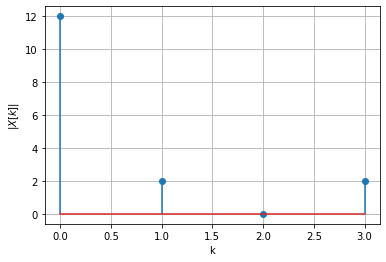
\includegraphics[width=0.9\columnwidth] {Gate_Assignment_1_Fig_1.png}
    \caption{Magnitude of $\vec{X}[k]$ vs $k$}
    \label{Magnitude of X[k]}
\end{figure}
\end{frame}

\begin{frame}
\begin{figure}[!ht]
    \centering
    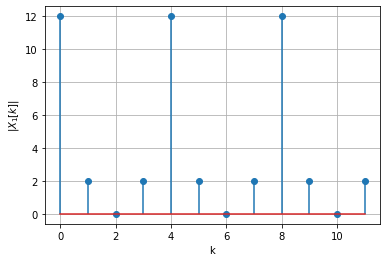
\includegraphics[width=0.9\columnwidth] {Gate_Assignment_1_Fig_2.png}
    \caption{Magnitude of $\vec{X_{1}}[k]$ vs $k$}
    \label{Magnitude of X1[k]}
\end{figure}
\end{frame}

\end{document}
